\documentclass[a4paper,11pt,utf8]{scrartcl}

\usepackage[ngerman]{babel}
\usepackage[utf8]{inputenc}
\usepackage[a4paper, left=2cm, right=2cm, top=1.5cm, bottom=1.5cm]{geometry}
\usepackage{graphicx}
\usepackage{stmaryrd}
\usepackage{listings}
\usepackage{amsmath}
\usepackage[hidelinks]{hyperref}
\usepackage[onehalfspacing]{setspace}

\setlength{\headsep}{.5cm}

\begin{document}

\pagestyle{empty}

% Titlepage
\noindent
Praktikum: Big Data \hfill Klemens Schölhorn, Sebastian Lange, Simon Hüning \hfill 11.03.2016\vspace{-.4cm}\\
\begin{center}
\huge\textsf{Lösungsskizze}\vspace{.1cm}\\
\large Publikationsanalyse auf den Daten der DBLP unter Verwendung von Apache Kylin
\end{center}

\section*{Einleitung}

Im ersten Abschnitt wird die Installation und Konfiguration von Kylin und der dafür benötigten Dienste auf dem Praktikumsserver beschrieben. Der zweite Abschnitt stellt das für die Analyse verwendete Datenbank-Schema vor. In den beiden darauf folgenden Abschnitte wird der Import und die Transformation der Daten und die anschließende Analyse in Kylin näher betrachtet. Dabei wird auch auf einige aufgetretene Probleme und Einschränkungen eingegangen. Das Dokument soll so die durchgeführten Arbeiten erläutern und bestimmte Entscheidungen während des Projektverlaufs nachvollziehbar machen.

\section{Server}

\subsection{Software}

Auf dem für das Praktikum zur Verfügung gestellten Rechner \texttt{wdi06} wurde basierend auf dem im installierten Ubuntu 14.04 LTS enthaltenen opendjk-7 folgende Software installiert:

\begin{itemize}
    \item Kylin: 1.2
    \item Hadoop (HDFS): 2.7.1
    \item HBase: 0.98.15
    \item Hive: 0.14.0
    \item Flink 0.10.1
\end{itemize}

\noindent
Es konnten aufgrund von Beschränkungen von Kylin\footnote{\url{http://kylin.incubator.apache.org/docs/install/index.html}} keine aktuellen Versionen von HBase und Hive verwendet werden. Es existiert zwar eine Version von Kylin für HBase 1.1.3, letzteres wurde jedoch noch nicht offiziell veröffentlicht.

\subsection{Einrichtung}

Die Hadoop-Umgebung wurde im pseudo-verteilten Modus installiert, d.\,h. es werden die gleichen Knoten wie in einer verteilten Umgebung verwendet, jedoch alle auf einer physischen Maschine und nur jeweils eine Instanz pro Knotentyp.

Die Installation erfolgte ohne root-Rechte in einem Benutzerverzeichnis durch Setzen der benötigten Umgebungsvariablen (\texttt{HADOOP\_HOME}, \texttt{HBASE\_HOME}, $\dots$). Dabei wurde weitgehend auf die Standard-Konfiguration gesetzt und nur die minimal benötigte Konfiguration vorgenommen.

Sämtliche Details zur Konfiguration (\texttt{README.md} und \texttt{INSTALL.md}), die für die Analyse entwickelten Programme und Skripte (\texttt{pub-importer} und \texttt{pub-formatter}), sowie dieses Dokument und die Abschlusspräsentation befinden sich in unserem Projektrepository\footnote{\url{https://github.com/klemens/bigdata-kylin-dblp}} bei GitHub.

\section{Datenbankschema}

Das folgende Sternschema basiert auf dem in der Aufgabenstellung vorgeschlagenen und wurde für die Verwendung in Kylin an einigen Stellen vereinfacht, da Kylin z.\,B. keine N:M-Beziehungen zwischen Fakten- und Dimensionstabellen unterstützt. Die Zitierungszahlen wurden direkt bei der Transformation durch Flink generiert.

\noindent
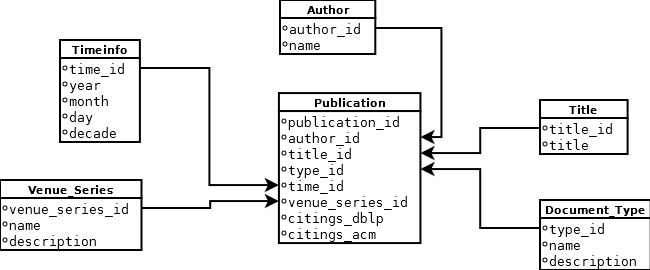
\includegraphics[width=\textwidth]{pics/Star-Schema-final}

\section{Datenimport und -Transformation}

Der Import der Daten gestaltete sich aufgrund der Datengröße schwierig. So kann die \texttt{dblp.xml} nicht direkt mit einem DOM-Parser verarbeitet werden, da dafür zu viel Speicher benötigt wird. Aus diesem Grund muss ein SAX- oder StaX-Parser verwendet werden.

Auch ein direkter Import per MapReduce stellte sich als schwierig heraus, da immer komplette XML-Records gelesen werden müssen, was der standardmäßig zeilenweisen Verarbeitung von MapReduce widerspricht. Hadoop besitzt zwar einen \texttt{StreamXmlRecordReader}, der jedoch selbst in aktuellen Versionen scheinbar nicht immer problemlos funktioniert\footnote{\url{https://issues.apache.org/jira/browse/MAPREDUCE-577}}.

Alternativ wird oft \texttt{XmlInputFormat} von Mahout (einem Hadoop-basierten Machine-Learning-Tool) verwendet\footnote{\url{http://oobaloo.co.uk/articles/2010/1/20/processing-xml-in-hadoop.html}}, was diese Probleme nicht hat. Allerdings müssen dabei alle zu lesenden Records das gleiche XML-Tag verwenden, was bei der \texttt{dblp.xml} leider nicht der Fall ist.

Aus diesem Grund haben wir ein eigenes Tool für den Import entwickelt. Der \texttt{pub-importer} liest die \texttt{dblp.xml} aus einer Datei oder von \texttt{stdin}, verwendet StAX für das Parsen und schreibt das Ergebnis anschließend direkt ins HDFS. Dabei ist unabhängig von der Größe der Eingabedatei der Speicherverbrauch konstant.

Die exportierten Daten werden dabei in einem zu Hive (oder alternativ zu unserem \texttt{pub-formatter}) kompatiblen Format geschrieben (CSV mit Backslash als Escape-Zeichen oder mit Anführungszeichen versehen) und bestehen aus zwei Dateien: Einmal die \texttt{Collections} wie Konferenzberichte oder Bücher und schließlich die \texttt{Publications} an sich mit entsprechenden Verweisen auf die \texttt{Collections}.

Zusätzlich kann der \texttt{pub-importer} auch den im Data-Warehouse-Praktikum verwendeten, unvollständigen xml-Dump von ACM lesen und auf die gleiche Weise ins HDFS schreiben. Da dort jedoch keine Informationen über die Journals enthalten sind, entfällt hierbei die \texttt{Collections}-Datei.

\subsection{Probleme bei der Datentransformation mit PDI}

Bei der Umsetzung der Datentransformation mit PDI kam es zu einigen Problemen. Ein Problem ist die Implementierung des OUTER-JOIN in PDI. Diese Implementierung arbeitet nicht wie erwartet. Dies könnte daran liegen, dass die OUTER-JOIN Logik ausschließlich als Merge-JOIN implementiert ist. Da sich dieses Problem mit einigem Aufwand umgehen lässt, ist die Umsetzung der Transformation mit PDI daran letztlich nicht gescheitert. Dafür jedoch an den folgenden Problemen.

PDI hat bei der Umsetzung stets sämtliche Schritte (Vergleich, Sortierung, Merge, etc.) parallel im Arbeitsspeicher ausgeführt. Es war daher auch mit 12 GB RAM nicht möglich alle Transformation auf der gesamten Datenmenge durchzuführen. Nach Laufzeiten von bis zu vier Stunden war das Ergebnis immer nur eine Exception. Für kleine Datenmengen hingegen funktionierte die selbe Transformation tadellos.

Darüber hinaus stellte sich während der Umsetzung heraus, dass die in PDI designten Transformationen nicht ohne weiteres auf dem Server ausführbar sind. Diese müssen (insofern kein zusätzlicher Deployment-Prozess dafür implementiert wird) auf dem Server immer an mehreren Stellen neu konfiguriert und angepasst werden, bevor sie ausführbar sind. Je komplexer die Transformation ist, umso umfangreicher sind die nötigen Anpassungen. Zusätzlich zu diesen Einschränkungen ist es alles andere als trivial, die Ausführung der Transformationen so zu konfigurieren, dass die Vorteile eines vorhandenen Clusters vollständig ausgenutzt werden.

Aus diesen Gründen ist das Verhältnis zwischen Aufwand und Nutzen sehr schlecht. Daher wurde die Datentransformation nicht, wie ursprünglich geplant, mit PDI umgesetzt.

\subsection{Datentransformation mit Apache Flink}

Nach den Problemen mit PDI wurde die Datentransformation in das Sternschema mittels Apache Flink implementiert, woraus dann der \texttt{pub-formatter} entstand.

Allerdings gab es auch hier einige Komplikationen: Das Problem ist die Verwendung von zwei verschiedenen CSV-Implementierungen, einmal der CSVReader von Apache Commons und dann der CSVReader von Apache Flink, wobei sich letzterer an keinerlei Standards (RFC 4180) hält und sich auch nicht ausreichend konfigurieren lässt. So unterstützt er nur die Quoting-Variante zum Speichern von CSVs. Allerdings erwartet er nicht wie üblich eine Verdopplung des Quoting-Zeichens, wenn dieses innerhalb eines Strings auftaucht, sondern erwartet das Escaping des Quoting-Zeichens mit einem Backslash, was weder dem Standard entspricht, noch mit dem CSVWriter von Apache Commons ausgegeben werden kann.

Abgesehen von diesem Problem läuft der Transformationsvorgang reibungslos. So werden zuerst die Dimensionstabellen erzeugt, indem die nötigen Felder aus den importierten Dateien in neue CSV-Dateien projiziert werden. Jeder Eintrag in den Tabellen ist dabei eindeutig. Die Faktentabelle entsteht anschließend durch einen Join der Dimensionstabellen. Der gesamte Vorgang dauert auf den dblp-Daten ca. zehn Minuten.

\subsection{Externe Hive-Tabellen}

Nach Abschluss des Transformationsprozesses mit dem \texttt{pub-formatter} werden auf den dabei erzeugten CSV-Dateien direkt externe Hive-Tabellen definiert, um den Zugriff aus Kylin heraus zu ermöglichen\footnote{Details zur Erstellung der Tabellen finden sich im Ordner \texttt{hql} in unserem Repository}.

\section{Analyse}

\subsection{Cube-Generierung mit Kylin}

Die Cube-Generierung erfolgt bequem über das Webinterface von Kylin. Es wurden im Verlauf des Praktikums mehrere Projekte mit verschiedenen Inhalten in Kylin angelegt. In jedem Projekt müssen als Grundlage für die Cube-Generierung zuerst die benötigten Hive-Tabellen hinzugefügt werden. Anschließend kann der Cube für die Datenanalyse konfiguriert werden. Die Cubes wurden dabei so entworfen, dass sie möglichst umfangreiche Analysen zulassen. Nach der Konfiguration wird der Cube dann von Kylin mit Hilfe von Map-Reduce-Jobs gebaut. Dies dauerte für die kompletten Daten der dblp ca. 80 Minuten. Der erzeugte Cube (in unserem Fall ca. 4 GiB groß) ist dann in einer HBase-Tabelle persistiert und kann direkt im Webinterface für die Analyse verwendet werden. Alternativ kann auch über eine SQL-basierte Schnittstelle darauf zugegriffen werden. Als Query-Engine kommt dabei Apache Calcite zum Einsatz.

\subsection{Analyse der Daten aus den Cubes}

Im Projekt lag der Schwerpunkt bei der Analyse der Daten nicht auf den Ergebnissen der einzelnen Abfragen an sich, sondern auf dem Vergleich der Ausführungszeiten der Abfragen, einmal basierend auf den in Kylin erzeugten Cubes und alternativ direkt in Hive. Es wurden verschiedene Abfragen entworfen, die bei Ausführung in Kylin immer die gleichen Ergebnisse lieferten wie bei der Ausführung in Hive. Diese Abfragen sind im Webinterface von Kylin im Bereich „Query“ als „gespeicherte Queries“ hinterlegt. Die Abfragen müssen zur Verwendung in Hive allerdings teilweise modifiziert werden, da der Funktionsumfang des Query-Interface von Kylin und von Hive unterschiedlich ist.

\subsection{Ergebnisse}

Die Analyse der DBLP Daten ergab, dass diese für eine Zitierungsanalyse ungeeignet sind. Die Daten enthalten prinzipiell nur wenige erfasste Zitierungen. Darüber hinaus sind die vorhandenen Verweise (z.\,B. verglichen mit Google Scholar) unvollständig. Zusätzlich wurde deutlich, dass die Daten für ältere Publikationen (vor 2000 publiziert) qualitativ und quantitativ deutlich besser erfasst sind, als für aktuellere. Im Bezug auf die Analyse von Zitierungen wäre es daher interessant, zukünftig eher Google Scholar als Datenquelle zu verwenden.

Hinsichtlich der Ausführungszeiten einzelner Abfragen ergab sich eine deutliche Beschleunigung bei Verwendung der mit Kylin erzeugten Cubes im Vergleich zu den Ausführungszeiten bei direkter Ausführung in Hive. Die in der Abschlusspräsentation dargestellten Werte sind jedoch nur als grober Identifikator für die Verbesserung der Performance bzgl. der Ausführungszeit der einzelnen Abfragen zu verstehen. Hier gibt es sowohl in Kylin, als auch in Hive mehrere Optimierungsmöglichkeiten, welche einen Einfluss auf die erhaltenen Messwerte haben können.

\section{Fazit}

Abschließend kann festgehalten werden, dass alle im Projekt verwendeten Technologien durchaus ihre Daseinsberechtigung haben, auch wenn es an der einen oder anderen Stelle noch Bugs oder fehlende Funktionen gibt. Die Auswertung der Ergebnisse zeigt, dass Kylin die Analyse der Daten deutlich beschleunigen kann. Eine Betrachtung noch ungenutzter Optimierungsmöglichkeiten, sowie ein Vergleich von Kylin mit einer ähnlichen Technologie wie z.B. Cloudera Impala, können spannende Aufgaben für die Zukunft darstellen.

\end{document}
